\chapter{Experiments}

\section{Benchmarks}

\subsection{Comparison of graph structures} \label{bench:graphStructure}
A benchmark was performed to compare the performance of a high level data structure and a byte stream (see table \ref{table:byteStreamHighLevelTime} and Figure \ref{fig:benchmarkByteStreamVsHighLevelMemory}). The graph in-2004 was used (see Appendix \ref{appendix4}). If all edges are added in one bulk, the performance measured will only reflect the complexity based on the input. By inserting the edges in bulks of 5000 both the complexity based on input and the existing structure is accounted for. The add time in table \ref{table:byteStreamHighLevelTime} is the time it takes to insert millions of edges in bulks of 5000. The iteration time is the time it takes to iterate over all edges in the graph once.

In figure \ref{fig:benchmarkByteStreamVsHighLevelMemory} the memory difference can be seen. The high level data structure and the byte stream have the same space complexity, but the difference can be explained by the memory overhead used by the high level data structure. 

\begin{table}[h]
    \center
    \begin{tabular}{ | l | l | l | l | l |}
        \hline
            & \multicolumn{2}{c}{Add time (s)} \vline & \multicolumn{2}{c}{Iteration time (s)} \vline \\ \hline
        edges             & High level & Byte stream & High level & Byte stream \\ \hline
        $10^6$            & 1.1        & 14.0        & 0.15       & 0.03 \\ \hline
        $2 \times 10^6$   & 2.3        & 47.4        & 0.29       & 0.04 \\ \hline 
        $3 \times 10^6$   & 3.5        & 100.1       & 0.40       & 0.05 \\ \hline
    \end{tabular}
    \captionsetup{justification=centering}
    \caption{Benchmark of representing the graph as a byte stream and a high level data structure}
    \label{table:byteStreamHighLevelTime}
\end{table}

\begin{figure}[h]
\centering
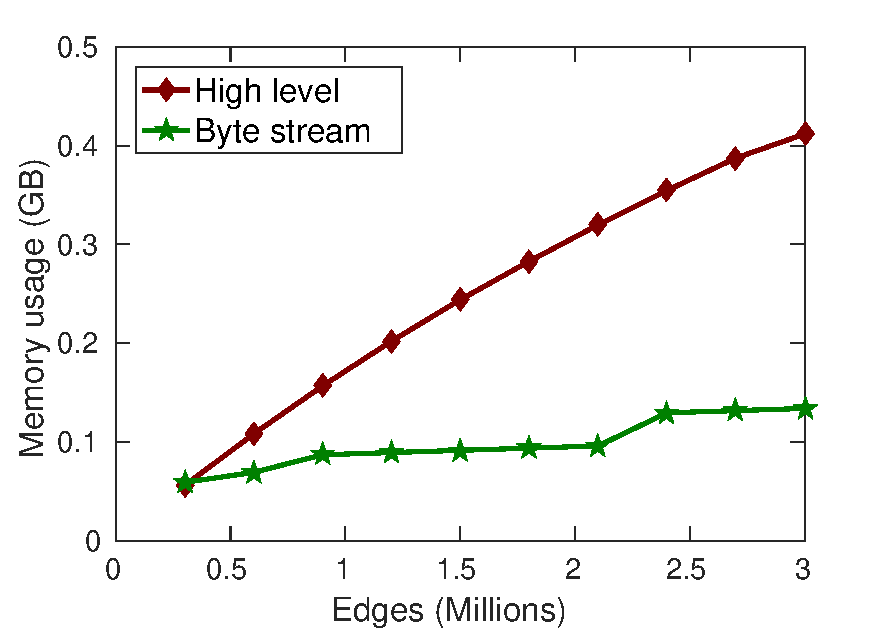
\includegraphics[]{benchmarkByteStreamVsHighLevelMemory}    
\captionsetup{justification=centering}
\caption {Benchmark of memory usage between high level structure and byte stream. }
\label{fig:benchmarkByteStreamVsHighLevelMemory}
\end{figure}


\subsection{Memory dependent merging} \label{bench:unionVsStored}
To find a suitable ratio $r$ between the memory used by the graph part saved as a byte stream and the part saved as a high level data structure, a benchmark was performed to compare the time and the space usage (see Figure \ref{fig:benchmarkUnionVsStored}). The benchmark was performed on the in-2004 graph (see Appendix \ref{appendix4}). 1,000,000 edges were randomly generated and inserted into the graph in bulks of 5,000. The measured time is the time to insert the edges into the dynamic graph and then to perform a complete edge scan. The measured memory is the graph's heap size. The plotted time values are the average of ten bulk insertions.

For reference, the benchmark compares a certain ratio $r$ with the extremes, $r = 0$ and $r = \infty$. With $r = \infty$ the additional entries are never merged with the original graph. This represents the optimal elapsed time. With $r = 0$, the graphs are always merged after each bulk insertion. This represents the optimal memory usage. By choosing $r = 8$, the benchmark shows that near optimality in both time and memory usage can be achieved. The graphs were made to visualize near optimality rather than trends.

\begin{figure}[h]
\centering
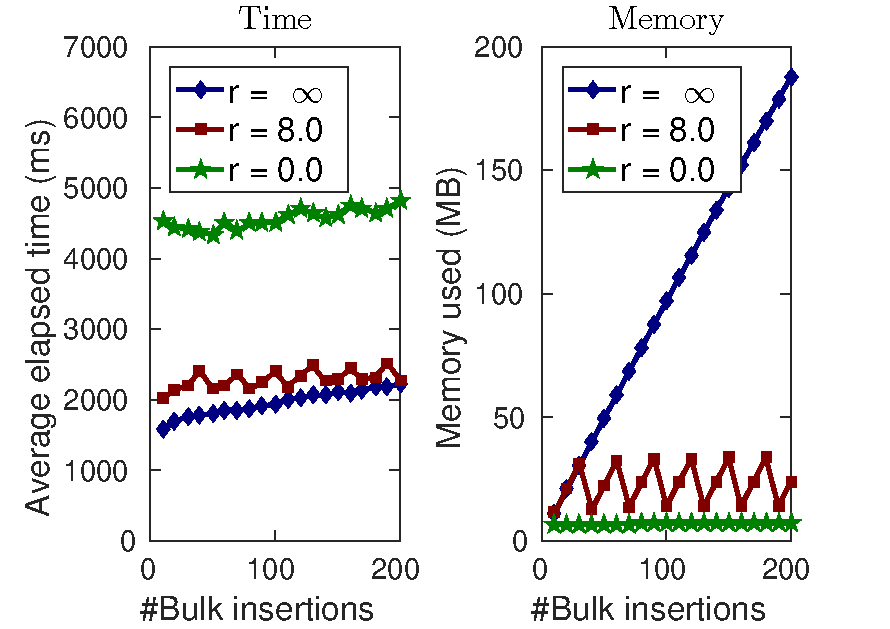
\includegraphics[]{benchmarkUnionVsStored}    
\captionsetup{justification=centering}
\caption {Benchmark of different union to stored memory ratio limits}
\label{fig:benchmarkUnionVsStored}
\end{figure}


\iffalse
\subsection{Comparison of different breadth-first search algorithms} \label{bench:msbfs}
A parallel standard BFS implementation and MS-BFS was compared by performing a benchmark (see Figure \ref{fig:benchmarkbfs}). Both algorithms had to perform breadth first searches from a certain number of source nodes and for a specified number of steps. The graph it-2004 (see Appendix \ref{appendix4}), was used. In figure \ref{fig:benchmarkbfs} the ratio between the total time for the standard BFS and the MS-BFS is plotted. Note that the y axis is logarithmic. The dashed line indicates where both algorithms are equally fast. MS-BFS is faster for all points above the dashed line and the standard BFS is faster for all points below it. From the figure it is clear that the standard BFS is faster for a small amount of steps but the speed ratio is exponentially increased in favor of MS-BFS as the steps increase. After $3$ steps, MS-BFS outperforms the standard BFS, even for a relatively small amount of sources. The standard BFS was up to $60$ times slower in our benchmark.

\todo{Add new plot and change text }
\begin{figure}[h]
\centering
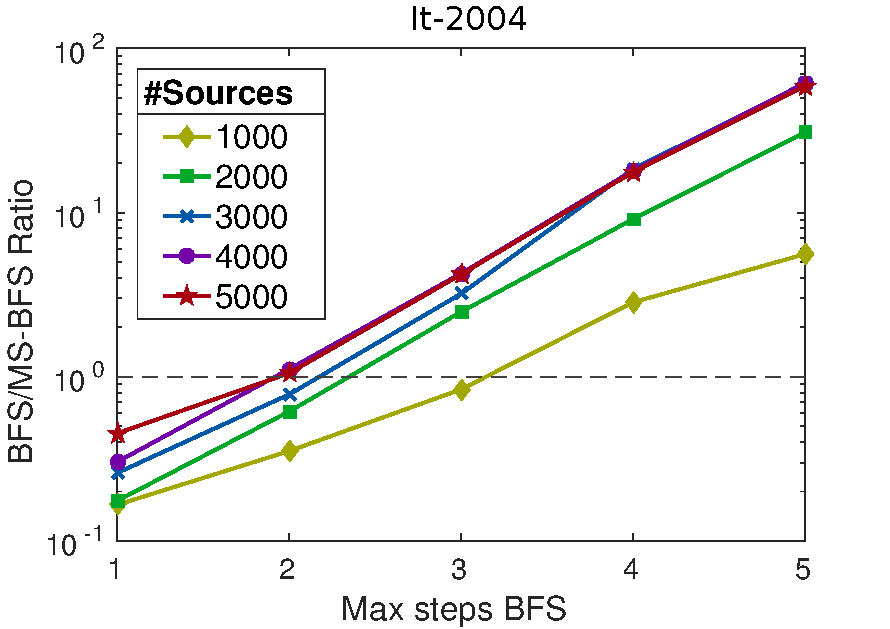
\includegraphics{benchmarkBfs}    
\captionsetup{justification=centering}
\caption {Benchmark of search time in parallel standard BFS and MSBFS}
\label{fig:benchmarkbfs}
\end{figure}
\fi

\subsection{Dynamic Vertex Cover} \label{bench:dvc}
The selected greedy algorithm was benchmarked with the it-2004 graph (see Appendix \ref{appendix4}). Starting with an empty graph, every edge was sequentially inserted from it-2004 into the dynamic vertex cover. Both the time and heap size was measured over the number of inserted edges (see Figure \ref{fig:benchmarkDvcInsertion}). This shows roughly 29.5 million inserted edges per second. The memory used mainly depends on the number of nodes. The heap size increased to 0.33GB implying an average of 8 bytes per node. 

\begin{figure}[h]
\centering
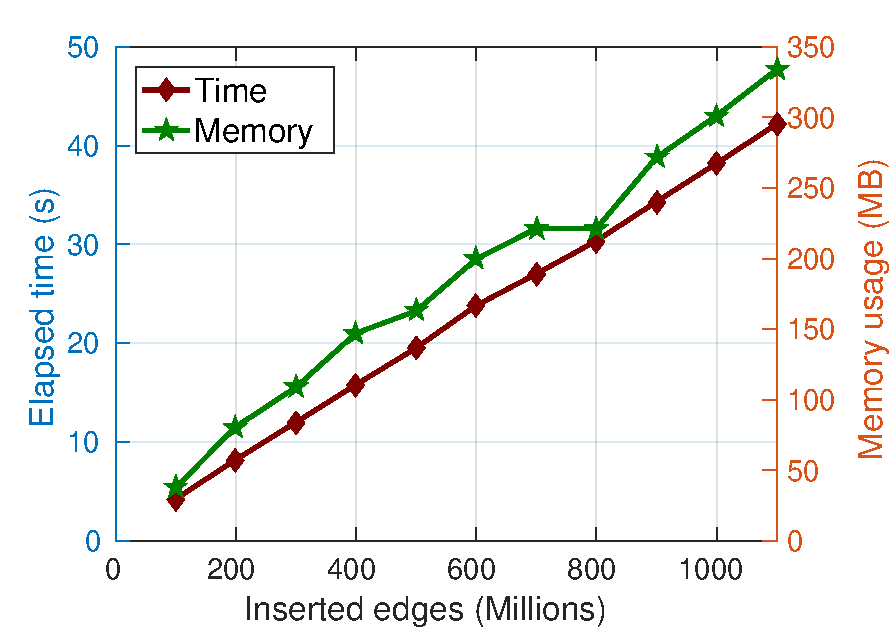
\includegraphics[]{benchmarkDvcInsertion}    
\captionsetup{justification=centering}
\caption {Benchmark of sequential insertions in 2-approximate dynamic vertex cover}
\label{fig:benchmarkDvcInsertion}
\end{figure}

To test the performance of sequentially deleting edges, the it-2004 graph was used (see Appendix \ref{appendix4}). The test was performed by first inserting all edges into the dynamic vertex cover and then sequentially deleting them (see Figure \ref{fig:benchmarkDvcDeletions}). All 1,150,725,436 edges were deleted in 220 seconds, giving a performance of 5,000,000 deleted edges per second. The heap usage is not plotted in the figure, as the algorithm is not designed to downsize the allocated memory for the vertex cover after deletions. 

\begin{figure}[h]
\centering
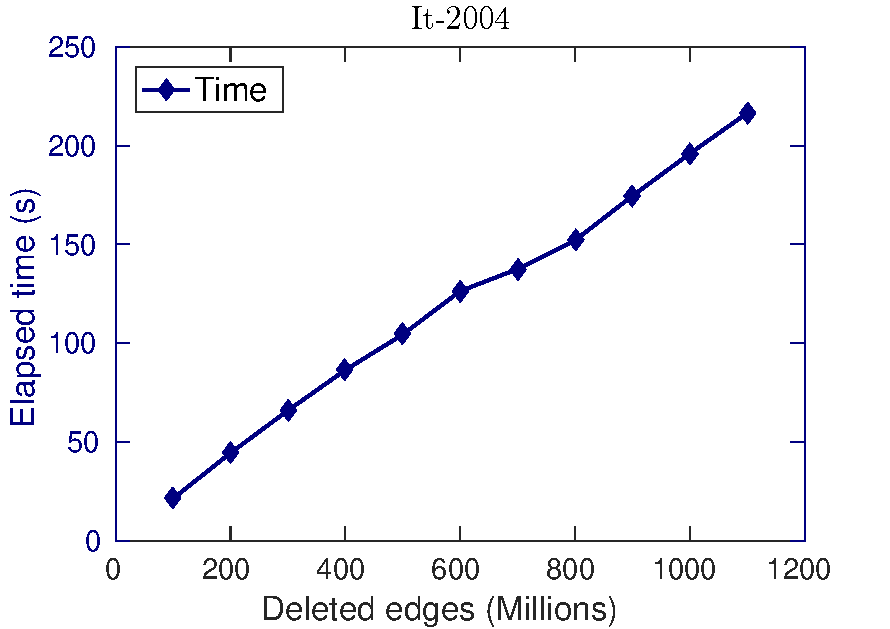
\includegraphics[]{benchmarkDvcDeletions}    
\captionsetup{justification=centering}
\caption {Benchmark of sequential deletions in 2-approximate dynamic vertex cover}
\label{fig:benchmarkDvcDeletions}
\end{figure}



\subsubsection{Comparison of unoptimized and final DANF}
A comparison between the two-BFS algorithm and DANF was performed by adding edges of different bulk sizes (see Figure \ref{fig:benchmarkDanfVsTrivial} and \ref{fig:benchmarkDanfVsTrivialh3}). The benchmark was performed on the graph in-2004 (see Appendix \ref{appendix4})  with 16 HyperLogLog registers per node for $h = 3$ and $h = 8$. The time measured was the time to insert random edges and update the counters. The memory usage of DANF was divided into the four main components while the two-BFS memory usage is for the complete algorithm. The figure shows that DANF scales with the edge insertions bulk size while the two-BFS algorithm's performance is constant. For large $h$-values DANF is up to 60 times faster than the two-BFS algorithm, but also uses up to 45 times more memory. For small $h$-values the gained speed of DANF is smaller but so is also the space consumption. Almost all of the memory used by DANF is used by MS-BFS. The vertex cover and graph space usage is almost too small to be seen in figure \ref{fig:benchmarkDanfVsTrivial}. 

\begin{figure}[h]
\centering
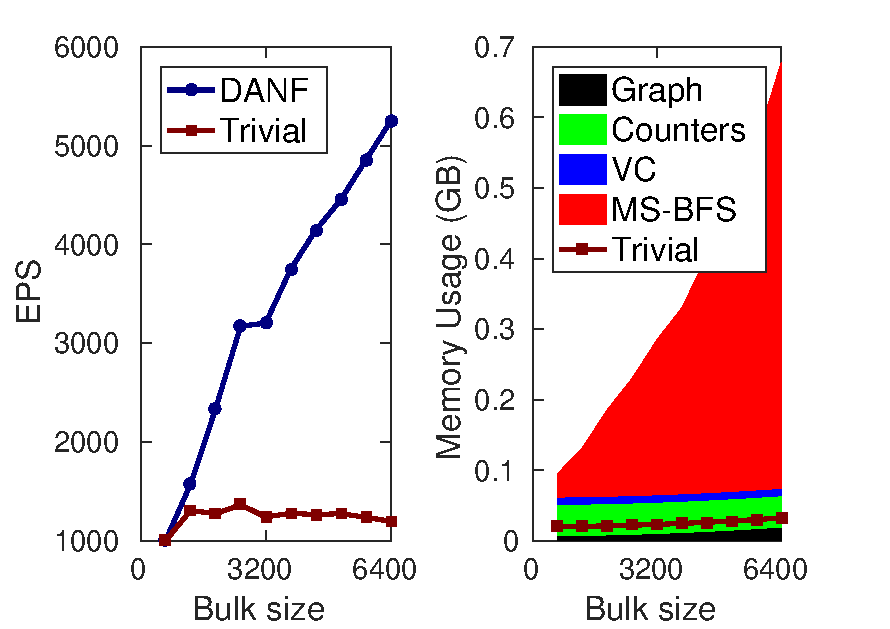
\includegraphics[]{benchmarkDanfVsTrivialh3}    
\captionsetup{justification=centering}
\caption {Benchmark of DANF and the two-BFS implementation with h = 3}
\label{fig:benchmarkDanfVsTrivialh3}
\end{figure}

\begin{figure}[h]
\centering
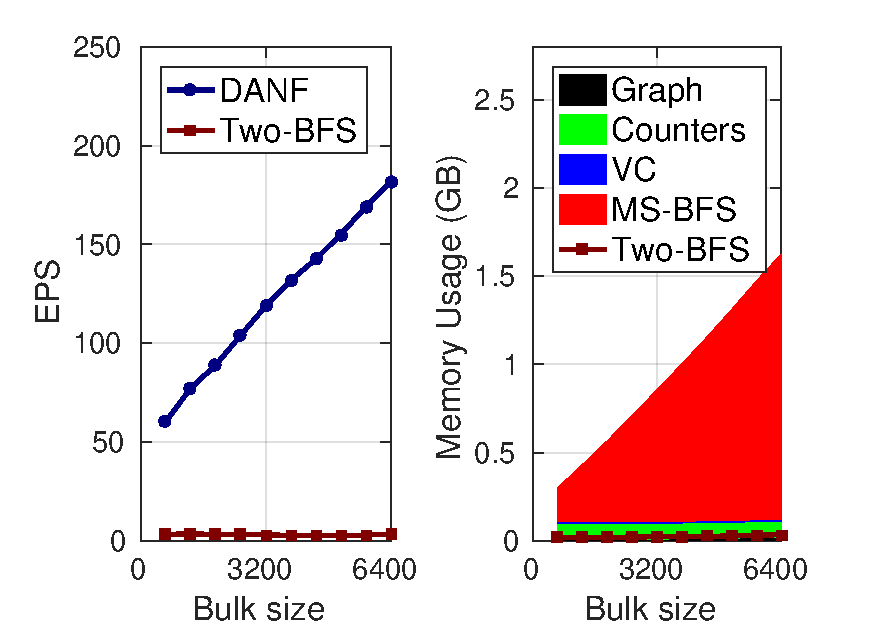
\includegraphics[]{benchmarkDanfVsTrivial}    
\captionsetup{justification=centering}
\caption {Benchmark of DANF and the two-BFS implementation with h = 8}
\label{fig:benchmarkDanfVsTrivial}
\end{figure}


\subsection{Comparison of DANF and HyperANF}
A comparison between DANF and HyperANF was made by inserting different amounts of edges into DANF. The number of added edges that was used as the limit was when the time of inserting the edges was the same as recalculating HyperANF. The graph in figure \ref{fig:benchmarkDanfVsHanf} shows the amount of edges added compared to the initial amount of edges. When the initial graph has 70.000 edges DANF can add more than the existing edges before HyperANF finishes the recalculation on the new graph, which is the sample right above $10^0$. However, when the initial number of edges increase the ratio of the total number of edges that can be added decrease. When the number of edges grows, DANF converge towards being able to add 0.01\% of the initial edges before a recalculation is completed. The ratio of added edges to initial edges decrease as $h$ increase.

\begin{figure}[h]
\centering
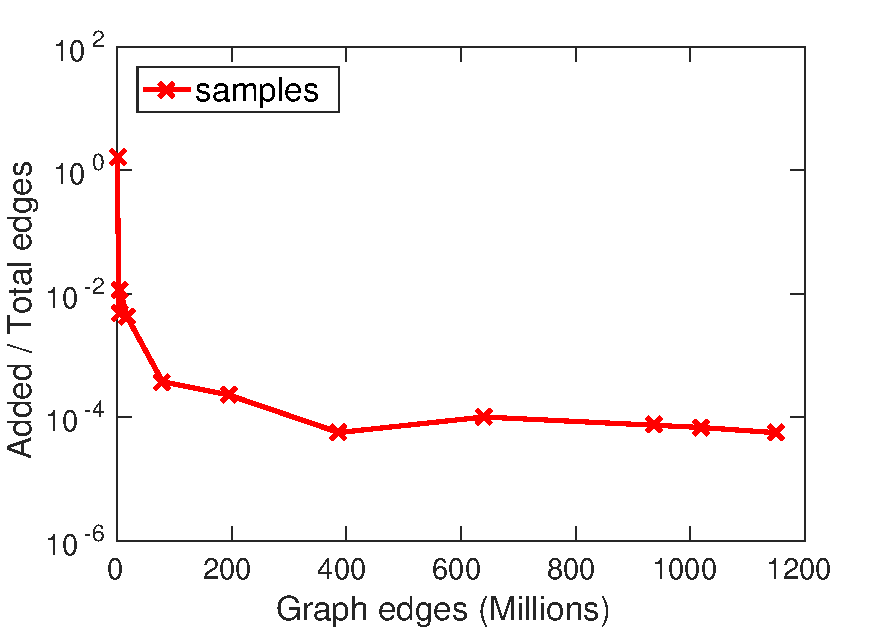
\includegraphics[]{benchmarkDanfVsHanf}    
\captionsetup{justification=centering}
\caption {Benchmark of the ratio of edges that can be added in the same time as a HyperANF recalculation with h = 3}
\label{fig:benchmarkDanfVsHanf}
\end{figure}

\subsubsection{MS-BFS tuning}
The MS-BFS article \cite{msbfs} mentions that if several MS-BFSs are to be performed the sources should be sorted and partitioned by out-degree. This increases the speed as when the sources have a higher out-degree, more BFSs meet and can join. When the number of edges added to DANF reaches a certain threshold, the insertions are divided into partitions. Sorting by out-degree improved the performance in the graph in-2004 (see Appendix \ref{appendix4}) by up to 37.2\% compared to no sorting. As it is preferable to make as many BFSs as possible to meet, sorting by the ANF value improves the performance even more. Sorting by the ANF value improved performance by up to 45\% compared to no sorting.   


\section{Experiments on a real-time data stream}

\begin{wrapfigure}{r}{0.4\textwidth}
  \begin{center}
    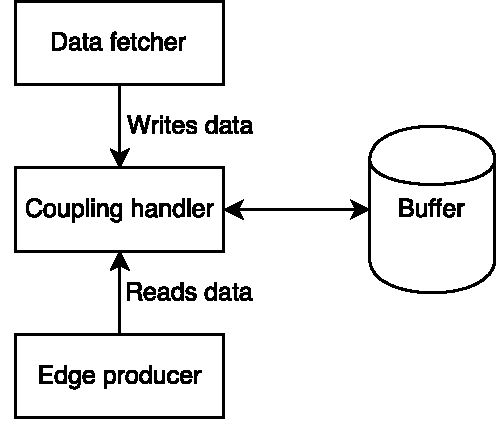
\includegraphics[width=0.38\textwidth]{Pipeline}
  \end{center}
  \caption{Parallel-compatible pipeline layout}
  \label{fig:pipeline}
\end{wrapfigure}

To do real-time experiments on a data stream, there are a few more tasks that need to be performed. The three main tasks are: fetch data, produce graph edges and update DANF. To efficiently perform these tasks they are run in parallel. They are implemented as components of a pipeline as seen in figure \ref{fig:pipeline}. A component stores its results in a buffer which can be read by the component next in the pipeline. The writing component has write-only access and the reading component has read-only access. Note that Edge producer can be a writer to a DANF updater using another coupling handler. This makes it possible to create a theoretically infinite pipeline with very low coupling between components and allows every component to run in their own threads.

As all nodes and edges are handled as plain numbers, a mapping needs to be stored from node index to the data. To avoid the data manager from competing with the algorithm for CPU and memory, the data should preferably be stored in a database by a completely different machine. The only data that needs to be saved on the same machine as the algorithm is a mapping from node index to data index, which can be saved on disk.

A list of the calculated value for each node is kept in a list $A$. Another list $B$ keeps track of the value of the nodes that change. After a given amount of time, the difference of the changed nodes are checked and nodes with significant changes are marked as rapidly changing. The elements in $B$ is added to $A$ and $B$ is cleared. This allows the detection of upcoming trends. 

Another useful feature used was to keep track of the top nodes, sorted in descending order according to their DANF values. Initially, all nodes were tracked. However, this turned out to be unsustainable on a graph with only a few millions of nodes. Instead, only the top most $X$ nodes were tracked. This leads to a drastic speed increase while still being able to check which are the most central nodes. 


\subsection{Graph layout}

When performing experiments on the data-stream a certain graph structure was used. The structure was designed to be able to detect popular subjects, authors and sources. This was achieved by creating three different graph models which, for simplicity, were combined into one (see Figure \ref{fig:experiment-graph}). The common node for all models is Document. 

The first model is the concept to document part. This model identifies popular subjects by retrieving all concepts that are mentioned in a document and then adding an edge from the concept to the document. The DANF value represents how many mentions a concept have. 

The second model is the location to document line in the middle. This model can identify which locations, sources (news) and authors that publishes the most documents.

The last model is the named entity part to the right in the figure. The named entities are general things mentioned in articles; such as countries, people or companies. Each entity has a sentiment. The sentiment specifies if the entity is mentioned in a positive (P), neutral (N) or negative (V) manner. Using the visualized structure for the named entities in figure \ref{fig:experiment-graph} enables detection of both the number of mentions and trends of how entities are referenced.

\begin{figure}[h]
\centering
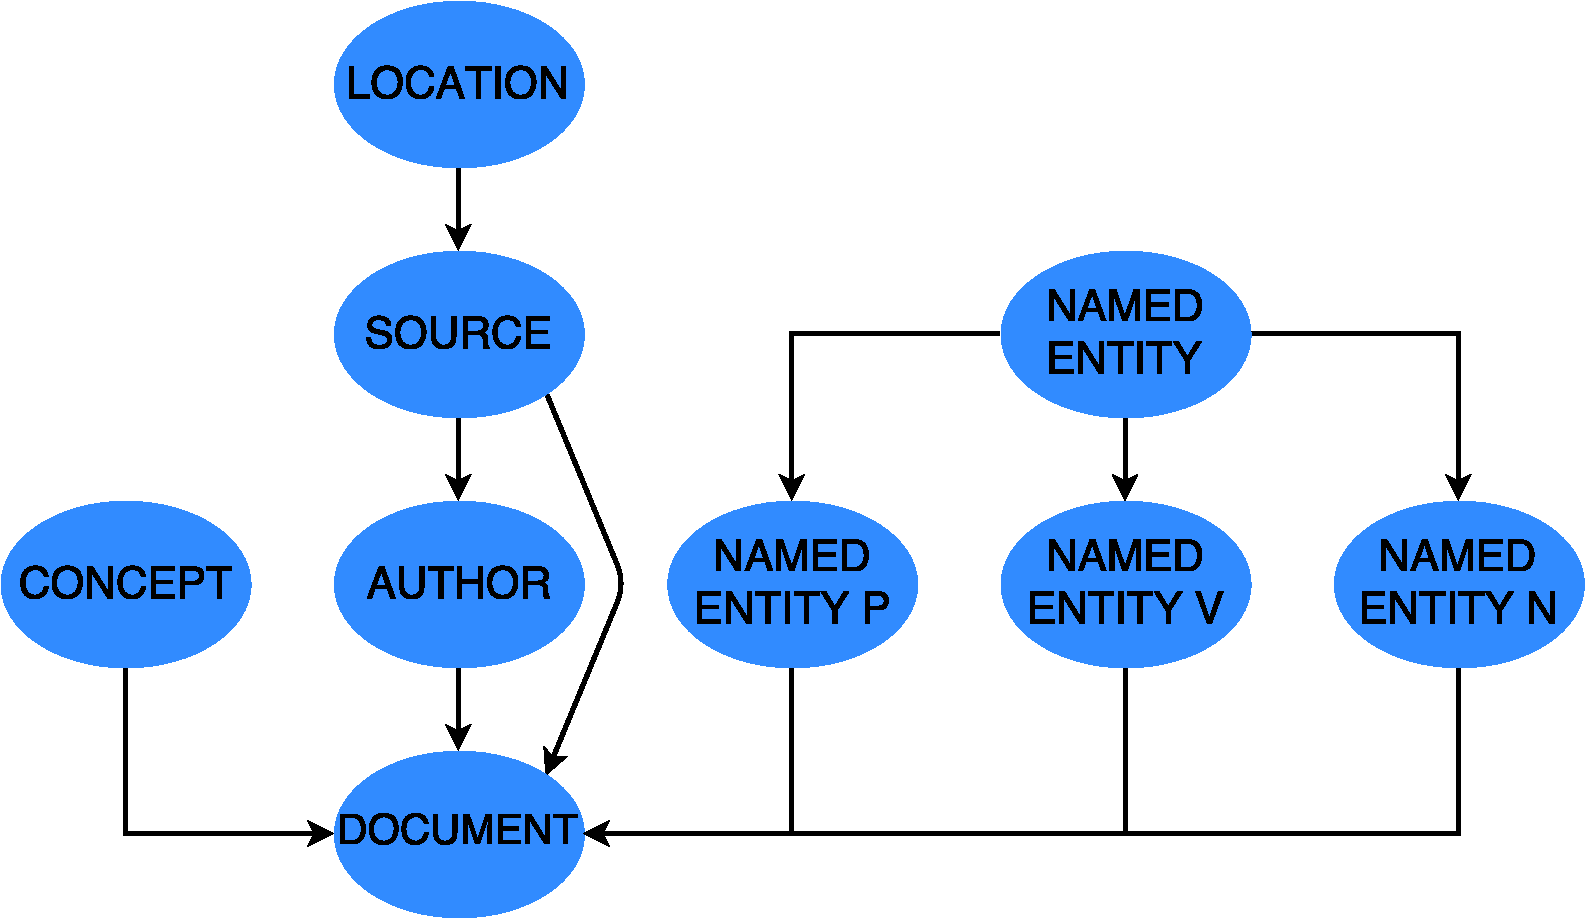
\includegraphics[width=\textwidth]{Graph}    
\captionsetup{justification=centering}
\caption {Graph layout used in the conducted experiment}
\label{fig:experiment-graph}
\end{figure}


\subsection{Starting with an empty graph}

The first experiment performed was done by creating an initially empty graph and setting up DANF to track the neighborhood function on it. A connection was established to the company live stream. The algorithm had no trouble keeping up with the stream of about 11 documents per second (two million documents per day) where about 30 edges were generated per document. 

\subsection{Starting with an arbitrary large graph}

Building a large graph from the existing data would take a long time. The data would have to be parsed and analyzed to generate edges. Instead of spending a large amount of time to generate the graph the it-2004 graph (see Appendix \ref{appendix4}), was used. DANF managed ten documents per second, which means that it could not quite keep up with the stream. This indicates that roughly one billion edges are the limit of the current implementation, but the it-2004 graph is more dense than the constructed graph so DANF would have a higher performance if the graph was made from scratch. More optimizations are required to prevent buffer build up in the long run. 

\subsection{Data retrieval}
From the experiment it was evident that both the United States and China were central nodes in the constructed graph. The United States was one of the most central node in all of the three models.

In the experiment, a trend concerning North Korea was detected. Short after North Korea released information concerning further nuclear tests, the DANF value of the North Korean concept node increased rapidly. Such trends can easily be detected by tracking rapidly changing nodes.
